\subsection{CPU Power Model is App Dependent}
\label{sec:primer_cpu}

%%% Things discussed in this section
%% 1. Explain the CPU architecture
%% 2. Explain how memory operation effects CPU model
%%   2a. Description of benchmark
%%   2b. What we did
%%   2c. Explanation of results
%% 3. Explain how CPU model is derived and generated
%%   3a. What did we do
%%   3b. How model is derived
%%   3c. Explain Base Current and Non-Base Current
%% 4. Explain the complete model

\paragraph{Parameters of a multicore CPU power model}
% 1. Explain the CPU architecture
Moto Z3~\cite{motoz3} is a representative modern smartphone
that uses the big.LITTLE CPU architecture~\cite{biglittlearch} to
provide energy efficiency in supporting diverse workloads.
% In this architecture, the CPU has two core clusters,
% the LITTLE cores with low compute performance and high power efficiency and
% big cores with high performance for processing compute-intensive tasks.
%The use of big.LITTLE cores depends on the dynamic usage pattern of smartphones i.e. when the phone is not working on doing any computationally intensive tasks it switches to LITTLE cores, dramatically extending the battery life.
% The cores in each cluster can run at various frequencies which correspond to 
% different core power states draining different amount of power.
In particular, in Moto Z3, the LITTLE cores can operate in 22 frequencies 
and big cores can operate in 31 frequencies.
%  The cores are switched to higher frequencies when higher performance is required.
At runtime, the OS scheduler along with the CPU governor performs power state transition and core frequency scaling to optimize the CPU energy drain as the workload varies.

Thus the parameters of the CPU power model include
the base power consumed $p_{base}$ when the cores are idle and
the non-base core $i$ power running at frequency $f_k$, $p^c_i(f_k)$, as listed in Table~\ref{tab:parameters}.
The total CPU power can be modeled~\cite{multicoremodel:2015} as follows:
\if 0
Accordingly, we model the CPU power draw as follows:
\begin{equation}
    P_{CPU} = p^c_{base} + \sum_i p^c_i{f(i)}
\end{equation}
where $p_{base}$ denotes the base power consumed when the cores are active and
$p_i{f_k}$ is the non-base power of core $i$ at frequency $f_k$.
\fi
{
\begin{equation}
    P_{CPU} = p^c_{base} + \sum_{i} p^c_i(f_k)
\end{equation}

}

\paragraph{TPMD methodology}
%% Flow of section
% 3. Explain how CPU model is derived and generated
%% 3a. What did we do
To derive the above CPU power model for Moto Z3,
we wrote a microbenchmark program that performs arithmetic-operations for 7 seconds at 100\% utilization followed by memory operations for 7 seconds at 100\% utilization. 
We ran the microbenchmark 10 times while fixing the big core cluster at each of the 31 frequencies, 
on 1 core, 2 cores and 4 cores.
When using 1 core, 2 cores and 4 cores, the remaining cores are offline.
We measure the base CPU power as the phone power draw when all cores are idle.
\footnote{We noticed even when the phone is idle, there are many system processes running in the background.
% 
So we obtained the accurate
base power from extrapolating the measured current vs. utilization curve for each frequency.}
We manually align the power monitor readings with each 7-second interval, 
and derive the non-base per-core power for each frequency by 
subtracting the base power from the measured total phone power.
{On Moto Z3, the per-core power $p_i(f_k)$ remains the same for different cores.}



% panab, check this ---
% The base CPU power is the current at utilization 0 and obtained from extrapolating the measured current vs utilization curve for each frequency.
% The non-base per-core CPU power for each frequency is the slope of the curve as shown in figure~\ref{fig:cpu_model_derivation}.

% at each big frequency.
% Little cores are offline
% Explain observations of microbenchmark

\if 0
\begin{figure}[tp]
    \centering
    \vspace{-0.1in}
         \begin{subfigure}[b]{0.49\columnwidth}
         \centering
         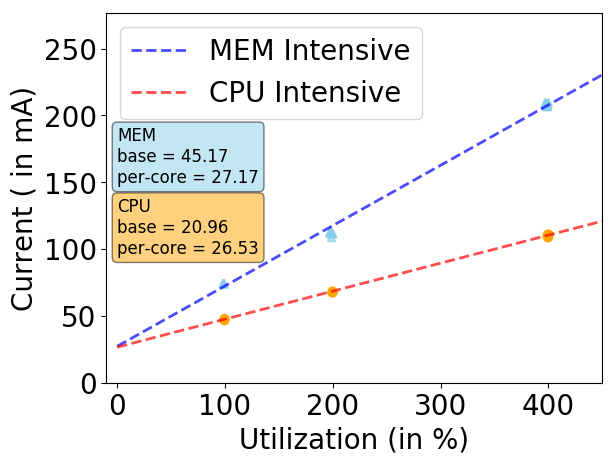
\includegraphics[width=\textwidth]{figures/576000.png}
         \caption{576 MHz}
         \label{fig:cpu_576000}
    \end{subfigure}
    \hfill
    \begin{subfigure}[b]{0.49\columnwidth}
         \centering
         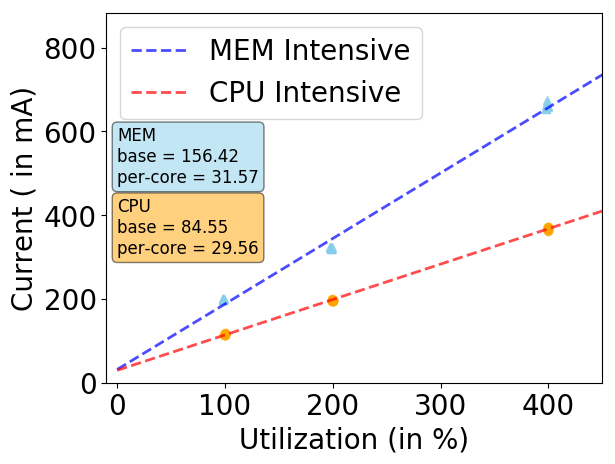
\includegraphics[width=\textwidth]{figures/1728000.png}
         \caption{1.728 GHz}
         \label{fig:cpu_1728000}
    \end{subfigure}
    \caption{The CPU derivation for two frequencies, 576 MHz and 1.728 GHz.}
    \label{fig:cpu_model_derivation}
    \vspace{-0.1in}
\end{figure}
\fi


\if 0
Figure~\ref{fig:cpu_model_derivation} shows 
the power consumed as a function of the CPU utilization for 576 MHz and 1.728 GHz,
for the two CPU benchmarks.
% While the blue line represents memory-intensive microbenchmark, red represents arithmetic-intensive microbenchmark .
% Figure~\ref{fig:cpu_576000} and~\ref{fig:cpu_1728000} corresponds to  576 MHz and 1.728 GHz
% Figure~\ref{fig:cpu_model_derivation} shows the power (averaged over 10 runs) linearly correlates with the utilization.
%% 3b. How model is derived
% We thus apply a regression-based solver to derive the best fit the following CPU power model:
% For each of the 31 frequencies, we derived a base and a per-core component with the following CPU power model.
% \begin{equation}
%     Power_{CPU}(f) = p_{base} + p_{f}*Utilization
% \end{equation}
% Where $p_{base}$ denotes the base power, and $p_{f}$ is the non-base per-core power running at frequency $f$.
%% 3c. Explain Base Current and Non-Base Current
For each of the 31 frequencies, we derived both base power and per-core component power.
We also observe that a reliable model can not be generated for the higher range of frequencies, like for frequencies higher than 2.035 GHz on MotoZ3 observations become unstable for CPU benchmarks.
The valid sets of base and per-core power were used for CPU modeling.
We observed that the base power is independent of frequency and per-core power is dependant on frequency.
Base power is 27.85 mA with a standard deviation of 1.22 mA.
% 
% We know the cores those are running at the 100\% utilization and remaining cores are offline.
% So, we can equate the number of running cores with utilization.
% We also observe that a reliable model can not be generated for the higher range of frequencies, like for frequencies higher than 2.035 GHz on MotoZ3 observations become unstable for CPU benchmarks.
% Fortunately, the apps rarely require these higher CPU frequency states and for our investigation we don't require those coefficients.
% \comment{stdev of what? fitting error on whole equation?}
% \comment{what is the following trying to say?}
During a  real run various cores may run on various frequencies.
\fi

\begin{figure}[tp]
    \centering
    \vspace{-0.1in}
         \begin{subfigure}[b]{0.49\columnwidth}
         \centering
    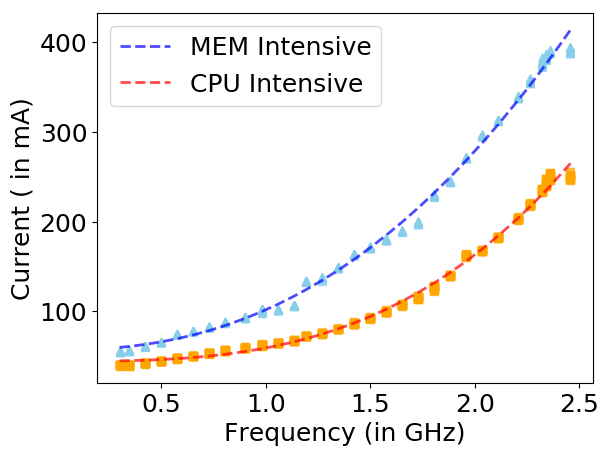
\includegraphics[width=\columnwidth]{figures/cpu_mem_characteristics.png}
    \caption{CPU power for compute-intensive vs. memory-intensive operations.}
    \label{fig:cpu_vs_mem}
\end{subfigure}
    \hfill
    \begin{subfigure}[b]{0.49\columnwidth}
         \centering
%    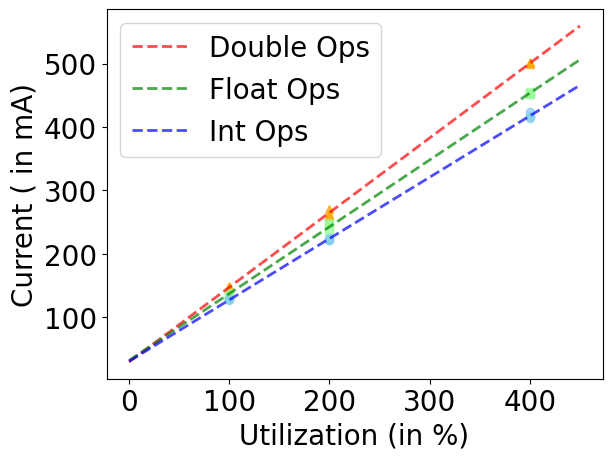
\includegraphics[width=\columnwidth]{figures/int_float_double.png}
    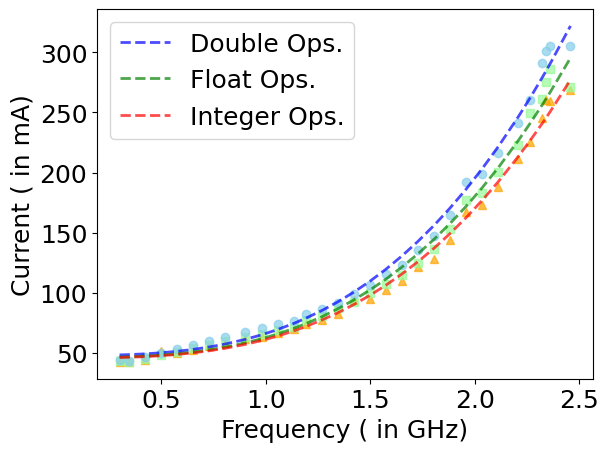
\includegraphics[width=\columnwidth]{figures/int_float_double_characteristics.png}
    \caption{CPU power for double, float and integer arithmetic operations.} % (for 1.8 GHz)}
    \label{fig:int_vs_float_vs_double}
    \end{subfigure}
    \caption{CPU power varies with app workload.}
    \label{fig:cpu_model_derivation}
    \vspace{-0.1in}
\end{figure}

\paragraph{Derived model}
Figure~\ref{fig:cpu_vs_mem} shows the derived CPU power model parameters
by plotting the total CPU power
as a function of the frequency.
% using the arithmetic-intensive and memory-intensive microbenchmarks. 
We observe that the CPU power draw for the two arithmetic-memory operation mix differ significantly,
by 38.7\% at the 300 MHz and 56.8\% at 2.45 GHz.
This suggests that the arithmetic-memory operation mix can send the CPU cores
to different power state variations draining different power.
In principle, this variation can be captured in the TPMD process by  
explicitly modeling memory as a separate phone component,
as in~\cite{carroll:2010,sesame:2011}, 
% gernot:2010 <- Koala: a platform for OS-level power management
using cache performance counter and free memory as the power triggers for memory draw. 
{
However, since the memory operation mix such as hardware counters is not collected by the mobile hardware 
or not reported by the Android OS on Android phones, it is much easier to lump memory power draw with CPU power draw as is commonly done in many recent work, including Android Battery Stats and Historian~\cite{androidbatterystats}. \comment{more example???}
}

Figure~\ref{fig:int_vs_float_vs_double} shows the derived CPU power model parameters for the integer only, 
float only, and double only arithmetic-intensive phases of the microbenchmark. 
We observe that the {CPU power} also differ, 
by 2.9\% at the 300 MHz and 13.5\% at 2.45 GHz.
This suggests that even the data type of arithmetic operations
can send the CPU cores into different power state variations.

\if 0
In summary, the above exercise of TPMD of CPU power shows the CPU power 
draw is very much app usage dependent and any fixed CPU model derived from
running a fixed microbenchmark is likely to have high estimation error when 
used in a particular app run. 
\fi


\if 0
\questionaj{This is not a very convincing argument. 1. For memory benchmark, is "CPU
power" = "CPU + memory" power? Or is the CPU power referenced in figure is true CPU 
power? If it is first, seeing higher "CPU power" is expected and not surprising.
2. Someone can argue that you could log memory triggers by instrumenting
compiler/libc/kernel,
why not just log?  Another paper didn't do it is not a strong reason. I think the 
argument we are trying to make is broader. That there are too many triggers that can 
affect a component power model. Because of which (a) micro-benchmark author may not 
know about all of them (b) building an exhaustive model could be expensive and not useful
as some model combinations may not even appear in real apps and (c) logging all 
triggers can be prohibitively expensive or not allowed. Because of this 
micro-benchmarks are hopelessly doomed.
If you agree,
we should also throw int-ops vs float-ops arithmetic, CPU temperature into the mix and use them to make the above three arguments.}
\fi